\section{Analysis}

CVS must be performance analyzed from three perspectives to fully understand the quality and limitations of the system.  First, CVS must be scalability analyzed to see how large the system can get in terms of users as well as file size.  CVS must then be analyzed for performance in terms of the space requirements as well as runtime requirements.

\subsection{Scalability Limits}

CVS puts an upper bound on the number of users that can use the system.  In order to label each sentence and paragraph with a 32-bit integer, CVS chooses to allocate 10 bits to identifying the user responsible for creating the sentence or paragraph, and the remaining 22 bits are for identifying the sentence or paragraph.  As a result, CVS supports at most 1,024 users, and each user can create at most approximately 4 million paragraphs.  Each paragraph can contain at most approximately 4 million sentences.  See Figure 1 for details.

\begin{figure}
\begin{center}
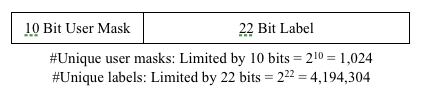
\includegraphics[scale=0.55]{analysis_figure_1.png}
\end{center}
\caption{Shows the structure of a sentence label as well as the arithmetic used to calculate the maximum number of users, sentences, and paragraphs.}
\end{figure}

\subsection{Space Analysis}

CVS requires space in implementation beyond the space necessary for storing the document for 2 reasons.  First, the system needs space to label each part of the document.  Then, the system needs to maintain a log of changes made.




\subsubsection{Labeling Overhead}

As noted above, labeling parts of the document will increase the length of the document by 32 bits for each sentence as well as 32 bits per paragraph.  Encoding each character using Unicode allocates 16 bits to each character.  Therefore each label effectively adds two characters, 32 bits, to the document.  Assuming the average paragraph has 10 sentences, CVS� labeling system effectively adds 22 characters per paragraph.  Since a paragraph has 872 characters on average, CVS labeling causes space overhead of 2.52\%.  See Figure 2 for details.

\begin{figure}
\begin{center}
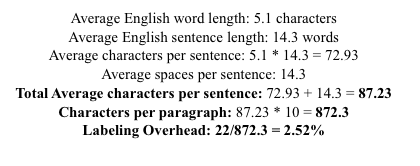
\includegraphics[scale=0.55]{analysis_figure_2.png}
\end{center}
\caption{Shows the arithmetic for calculating the labeling overhead.}
\end{figure}



\subsubsection{Logging Overhead}

As noted in Design, the log file holds information about how the file has changed since the last commit.  For the sake of analyzing the space required to log, we assume that since garbage collection happens every 30 seconds, users cannot make substantial changes to the document between garbage collection cycles.  Therefore, in the worst case, a user has changed every single sentence since the last commit.  This means that there is an entry in the log for each sentence.  Since a log entry is for all intents and purposes a sentence itself, the log is the size of the original file in the worst case.  In reality, the log is likely to be much smaller than the original file, but the space used has as upper bound the size of original file.

\subsection{Runtime Analysis}

CVS has two potentially runtime-intensive processes, which must be analyzed.  First, the process of merging is very computationally intensive.  It is additionally important to analyze the program's garbage collection process.

\subsubsection{Merging Runtime Analysis}

When two files merge, two processes must happen.  First, the program must determine where there are potential conflicts.  Then, the program must determine if a conflict actually exists.  All locations where a conflict exists are locations that the user must resolve himself.  Assume that the document has m sentences.  In the worst case, both users have changed all m sentences.  This means that each log has m entries.  In order to determine locations for potential conflicts, each entry of each log must be compared to each entry of the other log.  This amounts to m2 comparrisons in the worst case.  Since the document has only m sentences, only m conflicts must actually exist.  In order to test for conflict, the system must compare characters in each sentence.  Since a sentence has approximately 87 characters on average (see Figure 1), this amounts to 87*m operations.  That way, merging takes m2 + 87m operations in the worst case.  This is not unreasonable.  If we assume that a document has 10,000 sentences, which is an extreme case, as we expect documents to be smaller than this, merging will take 100,870,000 operations.  On a modern processor that can do 109 operations per second, that merge will take only 0.1 seconds.  See Figure 3.

\begin{figure}
\begin{center}
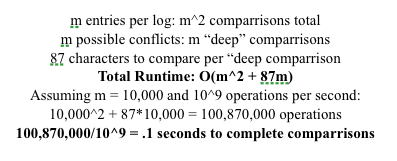
\includegraphics[scale=0.55]{analysis_figure_3.png}
\end{center}
\caption{Shows the runtime analysis of merge, as well as the arithmetic to determine the time in seconds.}
\end{figure}



\subsubsection{Garbage Collection Runtime Analysis}

Garbage collection takes place once every 30 seconds.  An element in the log is no longer necessary if that element is repeated later in the log.  To check for repeats, the log is backtracked, and each item is hashed.  If a collision occurs, the item causing the collision is removed from the log.  Therefore, garbage collection takes as long as it takes to iterate over the log.  Since we assume the log has in the worst case 10,000 entries, garbage collection should take 10,000 operations, which will take 1/105 seconds.